\documentclass[border=1cm]{standalone}

\usepackage{tikz}
\usetikzlibrary{shapes.geometric, shapes.misc}
\usetikzlibrary{cd, fit, calc}
\usetikzlibrary{positioning}
\usetikzlibrary{decorations.markings}
\usepackage{medl_colors}
\usepackage{graphicx} %package to manage images
\graphicspath{ {./images/} } 

\usepackage{arrayjob}
\def\words{{
{"Three","good","friends", "having", "fun"}
}}

\begin{document}
\begin{tikzpicture}

\foreach \i in {1,...,5}
{
    \pgfmathparse{int(\i-1)}\edef\j{\pgfmathresult};
    \pgfmathparse{\words[0][\j]} \edef\word{\pgfmathresult};
    \node[blueshape, rounded corners, minimum width=.5cm, minimum height=2cm] (unit\i) at (\j*2, 0) { };
    \node[rotate=90, below of=unit\i, node distance=0cm] {Unit};
    \node[above of=unit\i, node distance= 2cm] (word\i) {\large \texttt{\word}};
    \draw[-Triangle,uthickline] (unit\i) -- (word\i);

    \ifnum\i>1
        \draw[-Triangle,uthickline] (unit\j) -- (unit\i);
        \draw[-Triangle,uthickline, bend right, looseness=1.5] (word\j) to[out=90, in=-90] (unit\i.south);
    \fi
}

\node[lightgreenshape, trapezium, align=center, trapezium angle=80, minimum width = 2cm, shape border rotate=270, left of = unit1, node distance = 3cm ] (t1) {\Large  CNN };  

\node[scale = .07, left of = t1, node distance = 80cm] (inputpic)  {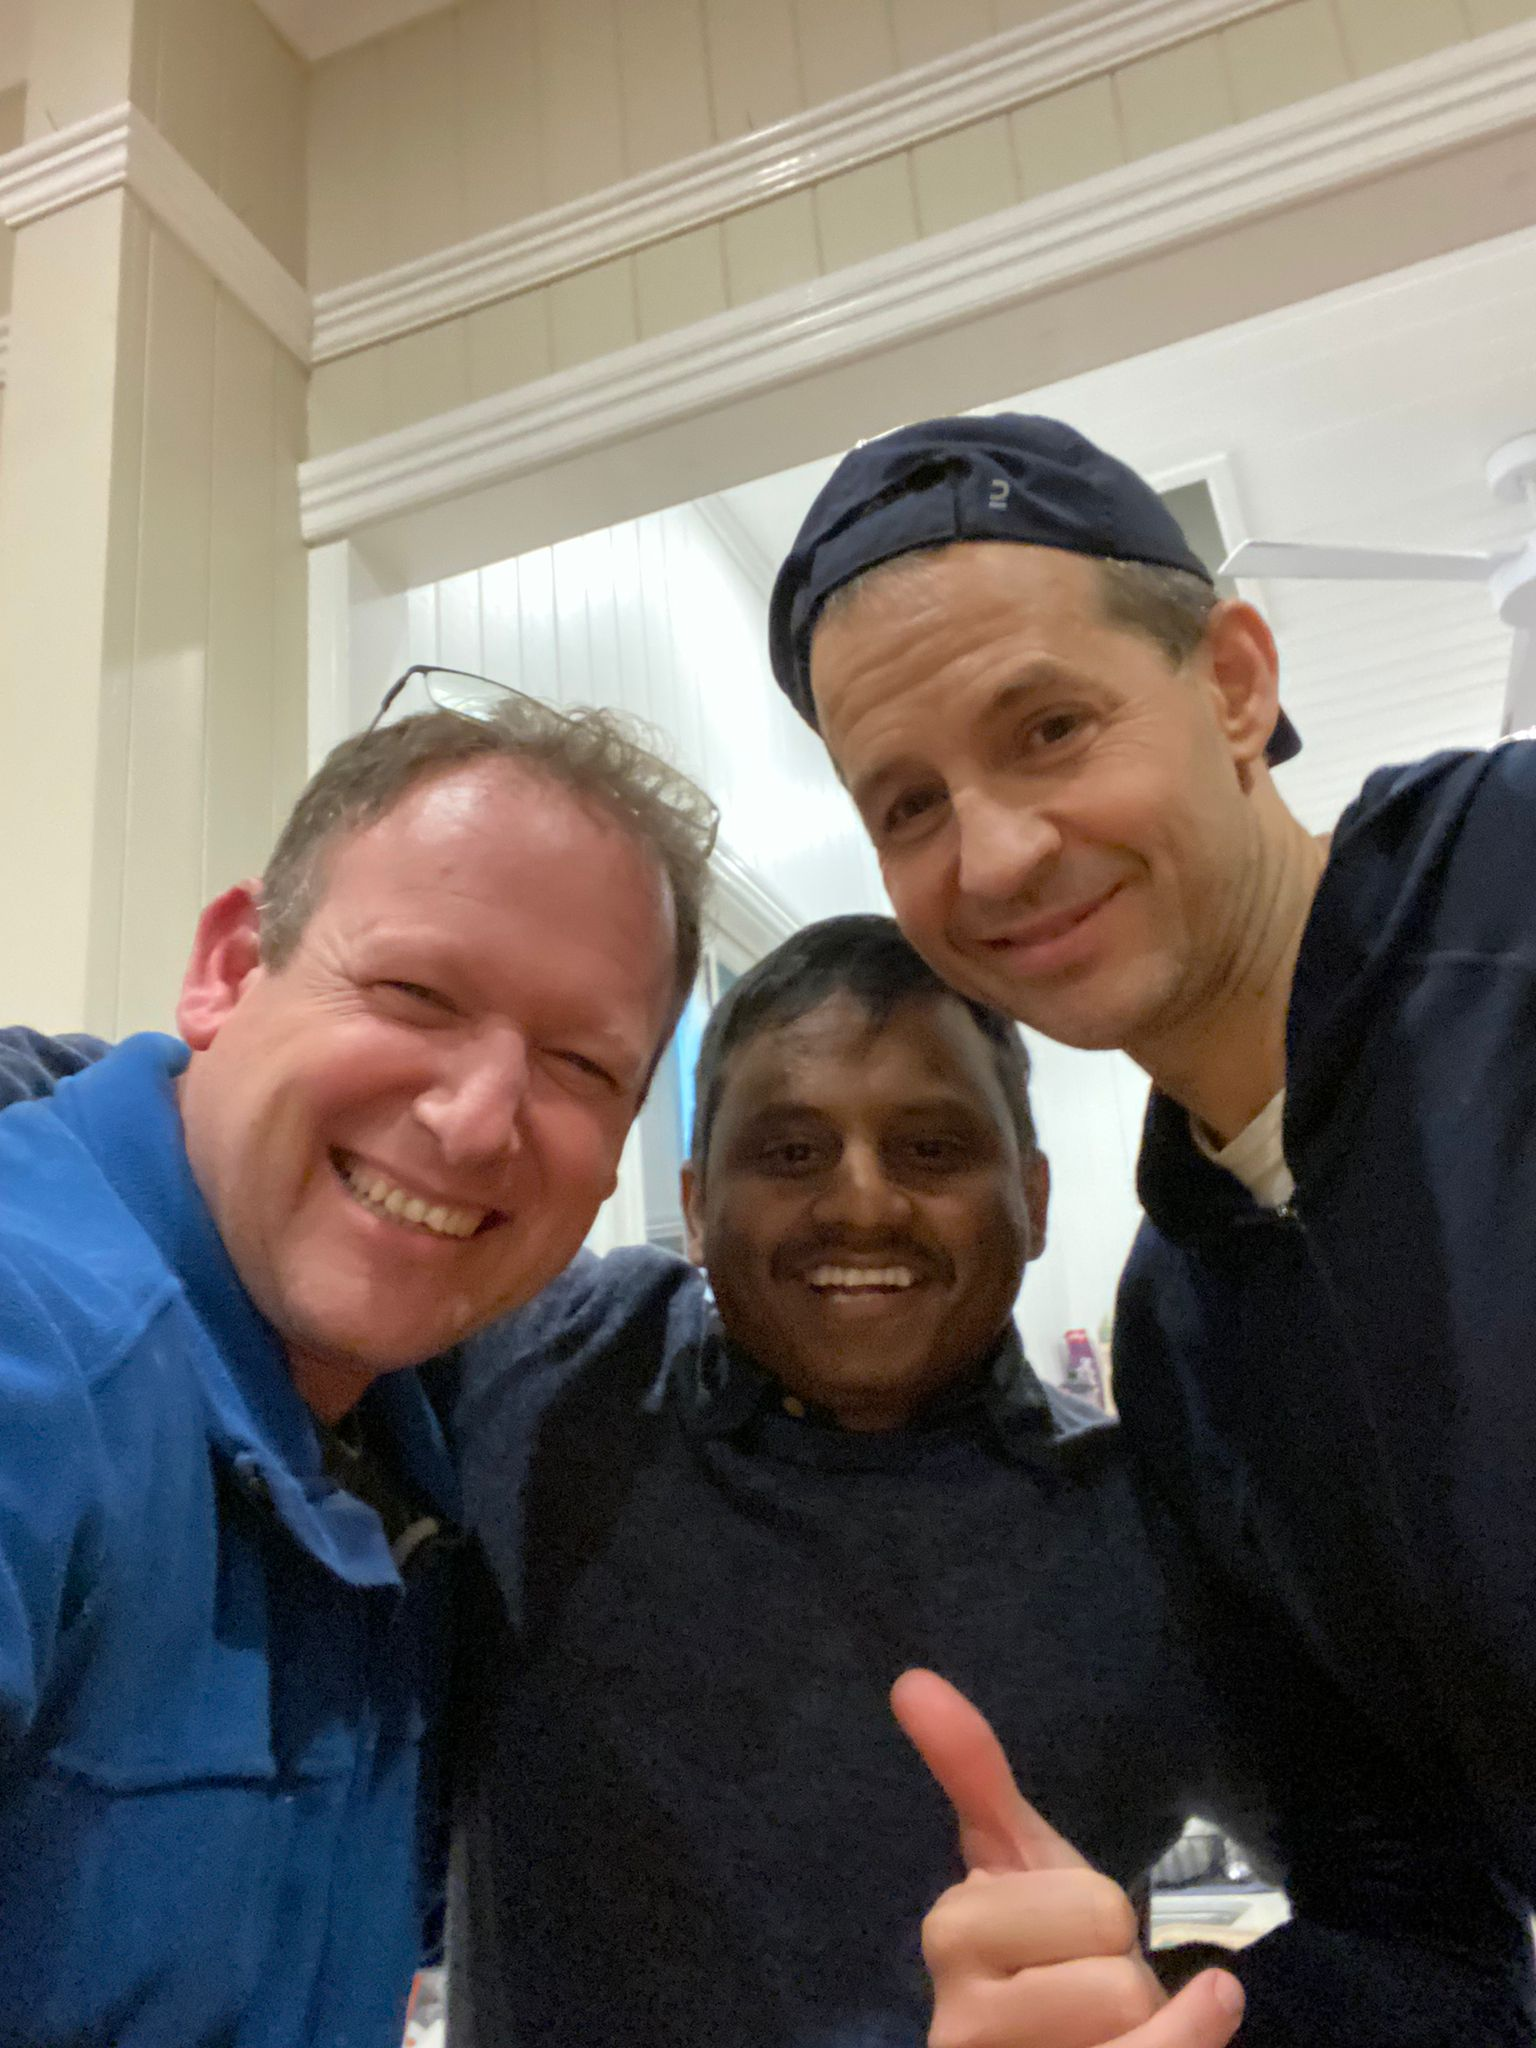
\includegraphics {images/threepersons.jpeg}};
\node[below of=unit1, node distance= 2cm] (word) {\large \texttt{<Start>}};

\draw[-Triangle,uthickline] (inputpic) -- (t1.west);
\draw[-Triangle,uthickline] (t1.east) -- (unit1);
\draw[-Triangle,uthickline] (word) -- (unit1);



\end{tikzpicture}
\end{document}
